\begin{problem}{3}
  Consider the family of functions $f_\lambda(x) = x^3 - \lambda x$ for some parameter
  $\lambda \in \mathbb{R}$.

  \begin{enumerate}
    \item Find all fixed points and determine their nature and where they
      are created as $\lambda$ varies.
    \item Find where a 2-cycle is created
      and give the graph of where this happens. Determine the stability of the
      hyperbolic 2-cycles.
    \item Use a graphing utility to find an approximate
      value of $\lambda$ where the 3-cycle is created. Give the graph of this situation.
  \end{enumerate}
\end{problem}

\begin{proof}
  \begin{enumerate}
    \item The fixed points of $f_\lambda$ are the roots of the function
      \begin{align*}
        g_\lambda(x) &= f_\lambda(x) - x\\
        &= x(x^2 - \lambda  - 1).
      \end{align*}
      Thus, the fixed points of $f_\lambda$ are $x_0 = 0$, $x_1 = \sqrt{\lambda + 1}$, and $x_2 = -\sqrt{\lambda + 1}$.
      Note that the points $x_1$ and $x_2$ are real only if $\lambda \geq -1$, i.e.\
      the points are only fixed points of the dynamical system if $\lambda \geq -1$.

      Using the first derivative of $f_\lambda$, we can classify the above fixed points
      when they are hyperbolic. If the fixed point is non-hyperbolic, we can use
      the second and third derivatives when the fixed point is non-hyperbolic
      of the type $f_\lambda'(x) = 1$, and the Schwarzian derivative when the fixed point is non-hyperbolic
      of the type $f_\lambda'(x) = -1$.      Note that
      \begin{align*}
        f_\lambda'(x) &= 3x^2 - \lambda \\
        f_\lambda''(x) &= 6x \\
        f_\lambda'''(x) &= 6.
      \end{align*}
      If $f_\lambda'(x) = -1$, we see that the Schwarzian derivative of $f_\lambda$ is given by
      \begin{align*}
        Sf_\lambda(x) &= -f_\lambda'''(x) - \frac{3}{2} \left[f_\lambda''(x)\right]^2 \\
        &= -6 - 54x^2.
      \end{align*}

      For the fixed point $x_0 = 0$, we see that $|f_\lambda'(x_0)| = |\lambda|$. Thus, the fixed point $x_0$ is
      a hyperbolic fixed point if $\lambda \neq -1$ or $\lambda \neq 1$. If $|\lambda| < 1$, then $x_0$ is asymptotically stable
      and if $|\lambda| > 1$, then $x_0$ is an unstable fixed point. If $\lambda = -1$, then $f_\lambda'(x_0) = 1$.
      Since $f_\lambda''(x_0) = 0$ and $f_\lambda'''(x_0) = 6 > 0$, the fixed point $x_0$ is unstable. If $\lambda = 1$,
      then $f_\lambda'(x_0) = -1$. The Schwarzian derivative of $f_\lambda$ at $x_0$ is then $Sf_\lambda(x_0) = -6 < 0$. Therefore,
      the fixed point $x_0$ is an asymptotically stable fixed point.

      Consider now the fixed point $x_1 = \sqrt{\lambda + 1}$ for $\lambda \geq -1$. We readily see that $|f_\lambda'(x_1)| = |3 + 2\lambda|$.
      If $\lambda > -1$, then $|f_\lambda'(x_1)| > 1$ and $x_1$ is
      hyperbolic and unstable. If $\lambda = -1$, then $x_1 = 0 = x_0$ and from the previous
      classification of the fixed point $x_0$, we know that $x_1$ is unstable.

      Lastly, consider the fixed point $x_2 = -\sqrt{\lambda + 1}$ for $\lambda \geq -1$.
      We thus have that $|f_\lambda'(x_2)| = |3 + 2\lambda|$ and the same classification for $x_1$ holds for $x_2$, i.e.\
      the fixed point $x_2$ is hyperbolic and unstable if $\lambda > -1$ and non-hyperbolic and unstable if $\lambda = -1$.

    \item Recall that a point $x$ is a period 2 point of $f_\lambda$ if $f_\lambda^2(x) = x$ and $f_\lambda(x) \neq x$. The 2-cycle associated to the period 2 point
      is then $\{x, f_\lambda(x)\}$. We thus look for solutions to the equation
      \begin{align}\label{period2}
        f_\lambda^2(x) - x &= \left(x^3 - \lambda x\right)^3 - \lambda \left(x^3 - \lambda x\right) - x \notag\\
        &= x^9 -3 \lambda x^7 + 3 \lambda ^2 x ^5 - \lambda ^3 x^3 - \lambda x^3 + \lambda^2 x - x \notag\\
        &= x (x^4- \lambda x^2 + 1)(x^2 - \lambda -1) (x^2 - \lambda + 1) = 0.
      \end{align}
      Suppose first that $\lambda < -1$. Then the only fixed point of the function $f_\lambda$
      is $x_0 = 0$ so that $x=0$ can be factored out of \eqref{period2} since the solutions we seek satisfy $f_\lambda(x) \neq x$. After factoring $x$ out from the above polynomial we have that
      \begin{align*}
        (x^4- \lambda x^2 + 1)(x^2 - \lambda -1) (x^2 - \lambda + 1) = 0.
      \end{align*}
      However, if $\lambda < -1$, then $(x^4- \lambda x^2 + 1) = 0$, $(x^2 - \lambda -1) = 0$,
      and $(x^2 - \lambda + 1) = 0$, all have no real solutions. Therefore, if $\lambda < -1$,
      then $f_\lambda$ has no period 2 points.

      Now consider $\lambda \geq -1$. Then for similar reasons we can factor $(x - x_0)(x - x_1)(x - x_2)$,
      where $x_i$ for $i=0,1,2$ are fixed points, out of \eqref{period2} and thus see that
      \begin{align*}
        (x^4- \lambda x^2 + 1)(x^2 - \lambda + 1) = 0
      \end{align*}

      To continue, we note that the first polynomial,  say $g(x) = x^4- \lambda x^2 + 1$, only has real solutions
      if $\lambda \geq 2$ and the second polynomial, say $h(x) = (x^2 - \lambda + 1)$, only has real solutions if $\lambda \geq 1$.
      Thus, for $-1 \leq \lambda < 1$ there are no period 2 points.

      If $1 \leq \lambda < 2$, then $h(x) = 0$ if $x = \pm \sqrt{\lambda - 1}$.
      Thus, $\{\sqrt{\lambda - 1}, - \sqrt{\lambda - 1}\}$ is a 2-cycle of $f_\lambda$.

      If on the other hand $\lambda \geq 2$, then $h(x) = 0$ has real solutions and the previous 2-cycle is still a 2-cycle
      of $f_\lambda$. However, $g(x) = 0$ also real solutions. These are given by
      \begin{align*}
        y_0 = -\frac{\sqrt{\lambda - \sqrt{\lambda^2-4}}}{\sqrt{2}}, \quad
        y_1 = \frac{\sqrt{\lambda - \sqrt{\lambda^2-4}}}{\sqrt{2}}\\
        y_2 = -\frac{\sqrt{\lambda + \sqrt{\lambda^2-4}}}{\sqrt{2}}, \quad
        y_3 = \frac{\sqrt{\lambda + \sqrt{\lambda^2-4}}}{\sqrt{2}}.
      \end{align*}
      Since $f_\lambda^2(y_0) = y_0$ and $f_\lambda(y_0) = y_3 \neq y_0$, we have that $\{y_0, y_3\}$ is an additional 2-cycle.
      Similarly, since $f_\lambda^2(y_1) = y_1$ and $f_\lambda(y_1) = y_2 \neq y_1$, we have that $\{y_1, y_2\}$ is the last 2-cycle.

      We now present the graphs of the bifurcation points $\lambda = 1$ and $\lambda = 2$ that indicate the
      birth of new 2-cycles in figure \ref{bif}.

      \begin{figure}[!h]
        \centering
        \begin{subfigure}{.45\textwidth}
          \centering
          \centerline{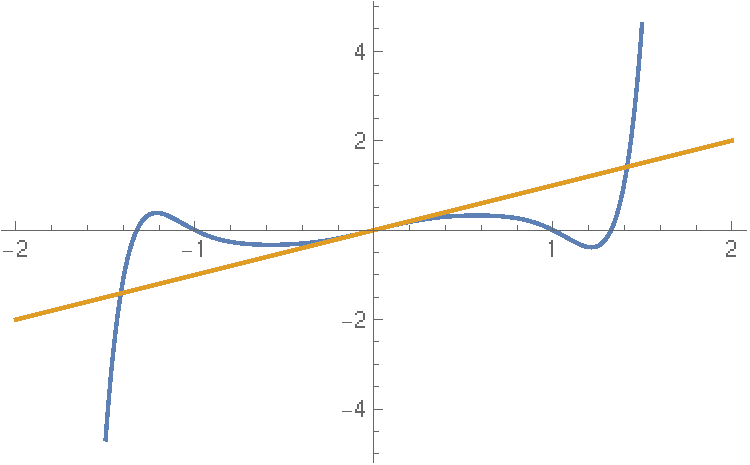
\includegraphics[scale=0.55]{bif_point_lambda_1}}
          \caption{The graphs of $f_\lambda^2(x)$ (blue) and $y=x$ (orange) for $\lambda = 1$.}
        \end{subfigure}
        \begin{subfigure}{.45\textwidth}
          \centering
          \centerline{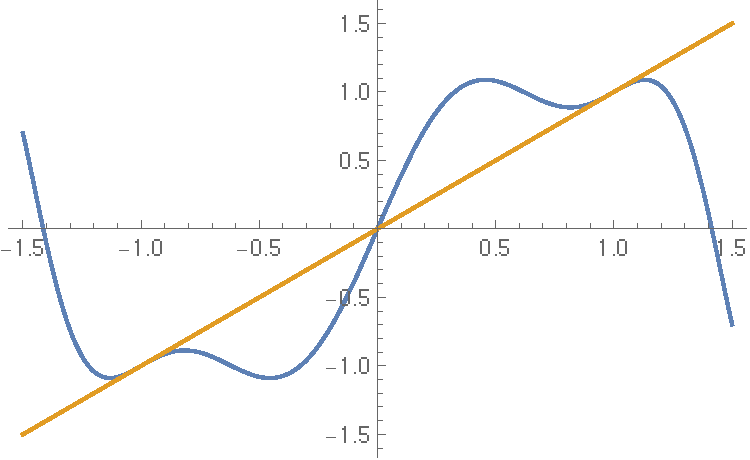
\includegraphics[scale=0.55]{bif_point_lambda_2}}
          \caption{The graphs of $f_\lambda^2(x)$ (blue) and $y=x$ (orange) for $\lambda = 2$.}
        \end{subfigure}
        \caption{The graphs of $f_\lambda^2$ at the bifurcation points $\lambda=1$ and $\lambda=2$ for the birth of 2-cycles. }
        \label{bif}
      \end{figure}

      In figure \ref{between}, we can see where the two cycles actually arise for values of $\lambda$ that occur
      between the bifurcations points $\lambda = 1$ and $\lambda = 2$.

      \begin{figure}[!h]
        \centering
        \begin{subfigure}{.45\textwidth}
          \centering
          \centerline{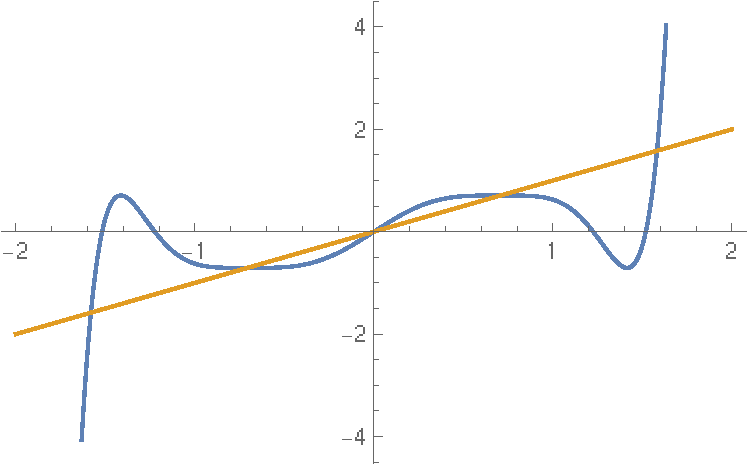
\includegraphics[scale=0.55]{lambda_gt1_lt2}}
          \caption{The graphs of $f_\lambda^2(x)$ (blue) and $y=x$ (orange) for $\lambda = 3/2$.}
        \end{subfigure}
        \begin{subfigure}{.45\textwidth}
          \centering
          \centerline{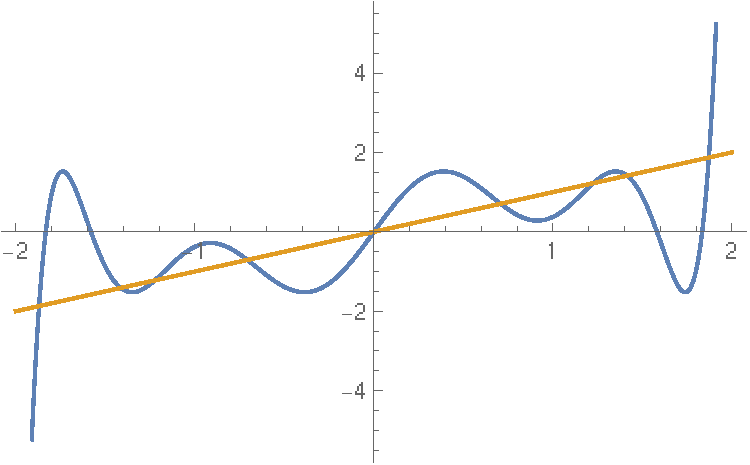
\includegraphics[scale=0.55]{lambda_gt2}}
          \caption{The graphs of $f_\lambda^2(x)$ (blue) and $y=x$ (orange) for $\lambda = 5/2$.}
        \end{subfigure}
        \caption{The graphs of $f_\lambda^2$ for values of $\lambda$ different from  the bifurcation points $\lambda=1$ and $\lambda=2$. }
        \label{between}
      \end{figure}

      We will now determine the stability of the hyperbolic two cycle $\{z_0, z_1\} = \{\sqrt{\lambda - 1}, -\sqrt{\lambda - 1}\}$ when $1 \leq \lambda < 2$
      and the stability of the hyperbolic two cycles $\{z_0, z_1\}$, $\{y_0, y_3\}$, and $\{y_1, y_2\}$ when $\lambda \geq 2$.

      Recall that for a function $g$ that a 2-cycle $\{z_0, z_1\}$ is hyperbolic and stable if
      $z_0$ is a stable fixed point of $g^2$, i.e.\ if
      \begin{align*}
        |(g^2(z_0))'| = |g'(g(z_0))g'(z_0)| = |g'(z_0)g'(z_1)| < 1.
      \end{align*}
      Note that $f_\lambda'(x) = 3x^2 - \lambda.$, Thus, we see  for the period 2 point $z_0$ that
      \begin{align*}
        \left|(g^2(z_0))'\right| &= \left|g'\left(\sqrt{\lambda - 1}\right)g'\left(-\sqrt{\lambda - 1}\right)\right| \\
        &= \left|\left(3\left(\sqrt{\lambda - 1}\right)^2 - \lambda\right)\left(3\left(-\sqrt{\lambda - 1}\right)^2 - \lambda\right)\right| \\
        &= \left|(2\lambda - 3)^2\right|.
      \end{align*}

      Similarly for the period 2 point $y_0$ we have that
      \begin{align*}
        \left|(g^2(y_0))'\right| &= \left|g'\left(-\frac{\sqrt{\lambda - \sqrt{\lambda^2-4}}}{\sqrt{2}}\right)g'\left(\frac{\sqrt{\lambda + \sqrt{\lambda^2-4}}}{\sqrt{2}}\right)\right| \\
        &= \left|\left(\frac{3\left(-\sqrt{\lambda^2 - 4} + \lambda\right)}{2}  - \lambda\right)\left(\frac{3\left(\sqrt{\lambda^2 - 4} + \lambda\right)}{2}  - \lambda\right)\right| \\
        &= \left|-2\lambda^2+9\right|
      \end{align*}
      and for the period 2 point $y_1$ we have that
      \begin{align*}
        \left|(g^2(y_1))'\right| &= \left|g'\left(\frac{\sqrt{\lambda - \sqrt{\lambda^2-4}}}{\sqrt{2}}\right)g'\left(-\frac{\sqrt{\lambda + \sqrt{\lambda^2-4}}}{\sqrt{2}}\right)\right| \\
        &= \left|\left(\frac{3\left(-\sqrt{\lambda^2 - 4} + \lambda\right)}{2}  - \lambda\right)\left(\frac{3\left(\sqrt{\lambda^2 - 4} + \lambda\right)}{2}  - \lambda\right)\right| \\
        &= \left|-2\lambda^2+9\right|.
      \end{align*}

      For the 2-cycle $\{z_0, z_1\}$ of $f_\lambda$,
      we see that $\left|(g^2(z_0))'\right| = \left|(2\lambda - 3)^2\right| < 1$ only if $1 < \lambda < 2$. Therefore, $\{z_0, z_1\}$
      is a hyperbolic, stable 2-cycle if $1 < \lambda < 2$.

      For the other 2-cycles $\{y_0, y_3\}$ and $\{y_1, y_2\}$, we see that
      $\left|(g^2(y_0))'\right| = \left|(g^2(y_1))'\right| = \left|-2\lambda^2 + 9\right| < 1$ only if
      $2 < \lambda < \sqrt{5}$. Therefore, it is for these values of
      $\lambda$ that the 2-cycles $\{y_0, y_3\}$ and $\{y_1, y_2\}$ are hyperbolic and stable.
    \item The plot in figure \ref{per3} shows that when $\lambda \approx 2.6995$, the graph
      of $f_\lambda^3$ touches the line $y=x$ at 6 points that differ from the fixed points of $f_\lambda$. Therefore,
      it is around this value of $\lambda$ that two 3-cycles occur for $f_\lambda$.
      \begin{figure}[!h]
        \centering
        \centerline{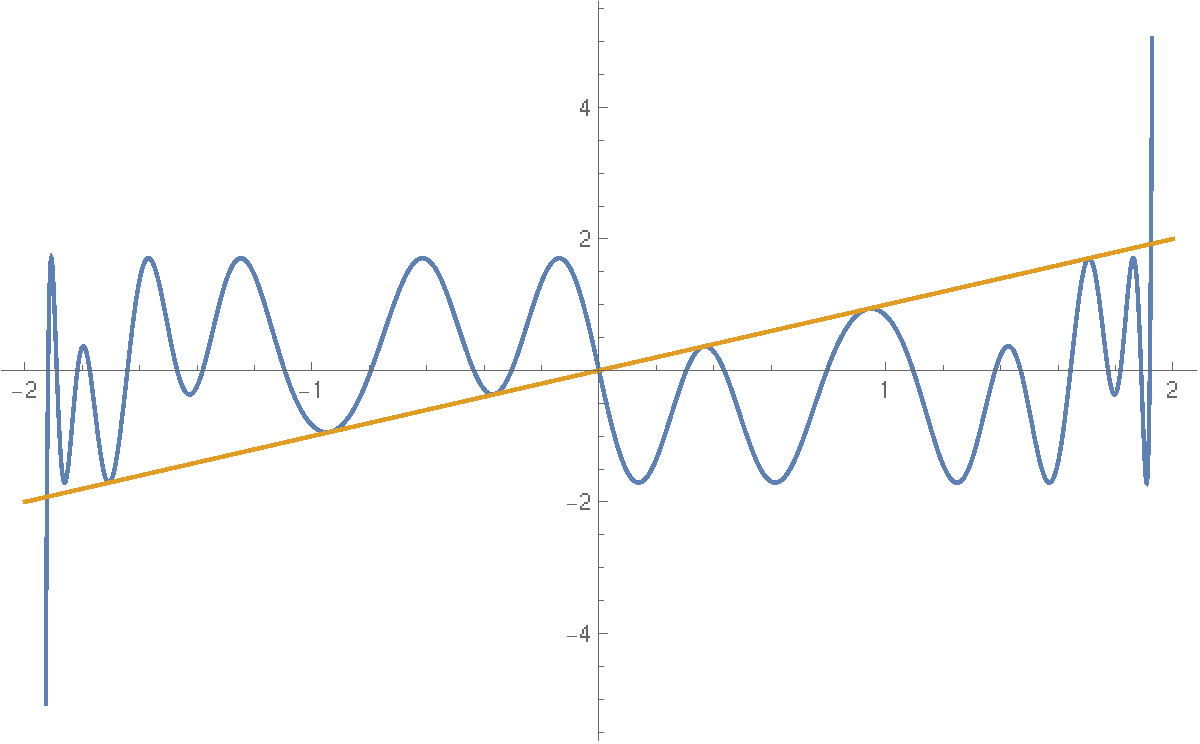
\includegraphics[scale=0.55]{period_3}}
        \caption{The graphs of $f_\lambda^3$ and $y=x$ for $\lambda= 2.6995$.}
        \label{per3}
      \end{figure}
  \end{enumerate}
\end{proof}
\newpage
